% Created 2021-02-15 lun 10:53
% Intended LaTeX compiler: pdflatex
\documentclass[presentation,aspectratio=169]{beamer}
\usepackage[utf8]{inputenc}
\usepackage[T1]{fontenc}
\usepackage{graphicx}
\usepackage{grffile}
\usepackage{longtable}
\usepackage{wrapfig}
\usepackage{rotating}
\usepackage[normalem]{ulem}
\usepackage{amsmath}
\usepackage{textcomp}
\usepackage{amssymb}
\usepackage{capt-of}
\usepackage{hyperref}
\usepackage{khpreamble}
\usepackage{amssymb}
\usepgfplotslibrary{groupplots}
\newcommand*{\shift}{\operatorname{q}}
\usetheme{default}
\author{Kjartan Halvorsen}
\date{2021-02-15}
\title{Actividad 1 - Retroalimentación \ldots{} y algo más}
\hypersetup{
 pdfauthor={Kjartan Halvorsen},
 pdftitle={Actividad 1 - Retroalimentación \ldots{} y algo más},
 pdfkeywords={},
 pdfsubject={},
 pdfcreator={Emacs 26.3 (Org mode 9.4.4)}, 
 pdflang={English}}
\begin{document}

\maketitle

\section{Resumen}
\label{sec:org8ffe32d}

\begin{frame}[label={sec:orge524404}]{Las instrucciones}
\begin{enumerate}
\setcounter{enumi}{2}
\item Identificar los \alert{componentes clave} del proceso
\item Identificar que \alert{variables físicas} se requiere conocer y/o monitorear para poder controlar el proceso.
\item Deducir componentes o \alert{acciones de control} requeridas
\item Elaborar el \alert{diagrama de bloques} de acuerdo a las funciones identificadas
\end{enumerate}
\end{frame}



\section{Ejemplo}
\label{sec:org99692d1}
\begin{frame}[label={sec:orgf608373}]{Sistema mecatrónico}
\begin{center}
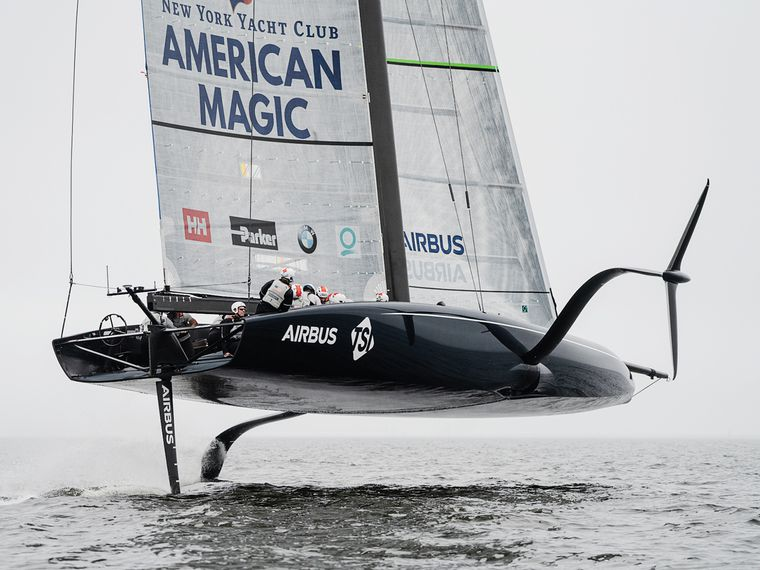
\includegraphics[height=0.7\textheight]{../../figures/ac75.jpeg}\\
{\footnotesize  From SailingWorld}
\end{center}

\href{https://www.sailingscuttlebutt.com/wp-content/uploads/2018/03/AC75\_Class\_Rule.pdf}{AC75 Class rule}
\end{frame}


\begin{frame}[label={sec:orgcc77b50}]{sistema de hidroalas}
 \begin{center}
\includegraphics[height=0.6\textheight]{../../figures/ac75-lines.png}
\includegraphics[height=0.7\textheight]{../../figures/ac75-class-foil.png}\\
{\footnotesize  by françois chevalier \hfill from the ac75 class rule}
\end{center}
\end{frame}

\section{Análisis}
\label{sec:org48915d9}

\begin{frame}[label={sec:orgd06e813}]{3. Componentes claves}
\begin{center}
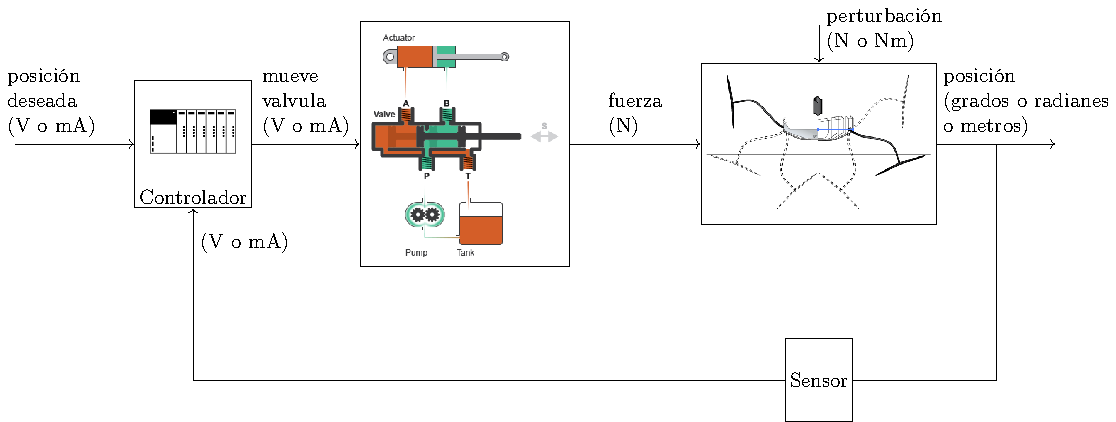
\includegraphics[width=.8\textwidth]{../../figures/ac75-control-block-feedback-units}
\end{center}

\begin{itemize}
\item \alert{Proceso} Aquí es un \alert{sistema mecanico} o \alert{mecanismo}
\item \alert{Actuador} Conversión de una señal de información a fuerza/torque/flujo/energía
\item \alert{Sensores}  Conversión de una variable física a una señal de información
\item \alert{Controlador} Computadora o microcontrolador o PLC, recibe señales, ejecuta el algoritmo de control, manda acción de control (señales) a los actuadores.
\end{itemize}
\end{frame}


\begin{frame}[label={sec:orgca93bde}]{4. Variables físicas}
\begin{columns}
\begin{column}{0.5\columnwidth}
\begin{center}
\includegraphics[height=0.8\textheight]{../../figures/ac75-class-foil.png}
\end{center}

{\footnotesize from the ac75 class rule}
\end{column}
\begin{column}{0.5\columnwidth}
\begin{center}
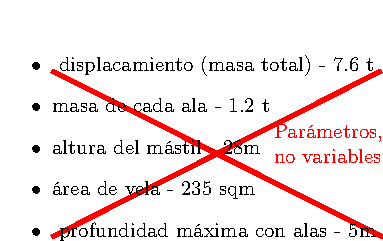
\includegraphics[width=0.8\textwidth]{../../figures/parameters-not-variables}
\end{center}
\end{column}
\end{columns}
\end{frame}

\begin{frame}[label={sec:orgdb6c4df}]{4. Variables físicas}
\begin{columns}
\begin{column}{0.5\columnwidth}
\begin{center}
\includegraphics[height=0.8\textheight]{../../figures/ac75-class-foil.png}
\end{center}

{\footnotesize from the ac75 class rule}
\end{column}
\begin{column}{0.5\columnwidth}
\begin{itemize}
\item Posición continua de los pistones (implicando posición del ala)
\item Presión hydraulica
\item Estado de cargo de las pilas
\end{itemize}
\end{column}
\end{columns}
\end{frame}


\begin{frame}[label={sec:org972f843}]{4. Variables físicas}
\begin{columns}
\begin{column}{0.3\columnwidth}
\textbf{Presión}
\begin{center}
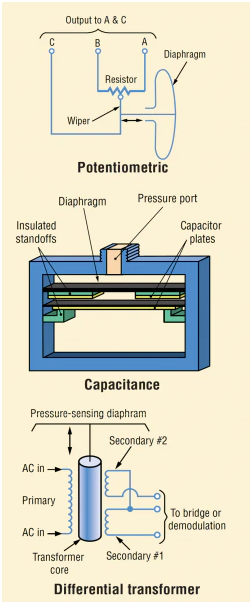
\includegraphics[width=0.67\linewidth]{../../figures/pressure-sensor.png}\\
{\footnotesize Fuente: Hydraulics \& Pneumatics}
\end{center}
\end{column}

\begin{column}{0.7\columnwidth}
\textbf{Posición}
\begin{center}
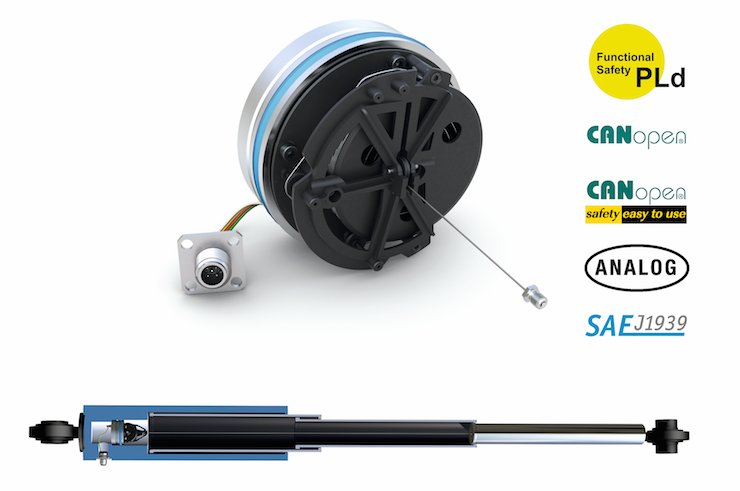
\includegraphics[width=0.7\linewidth]{../../figures/PosSensor.png}\\
{\footnotesize Fuente: Fischer Christian SIKO GmbH}
\end{center}
\end{column}
\end{columns}
\end{frame}
\begin{frame}[label={sec:org0d152db}]{5. Acciones de control}
La señal de entrada principal al sistema es la posición deseada del brazo/ala. La questión es \alert{¿como mover y mantener el brazo a la posición deseado?}
\end{frame}

\begin{frame}[label={sec:orgcf65506}]{5. Acciones de control - actuador}
\begin{columns}
\begin{column}{0.5\columnwidth}
\begin{center}
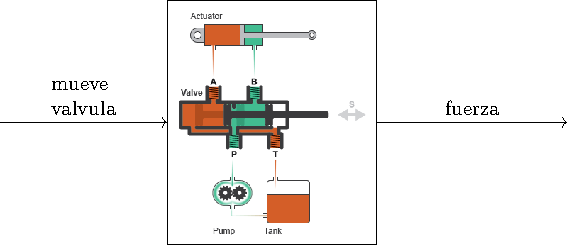
\includegraphics[width=0.9\textwidth]{../../figures/ac75-control-actuator-only}\\
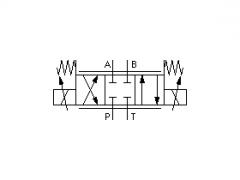
\includegraphics[width=0.8\textwidth]{../../figures/43-valve-proportional.jpg}
\end{center}

{\footnotesize Fuente: Festo}
\end{column}

\begin{column}{0.5\columnwidth}
\begin{center}
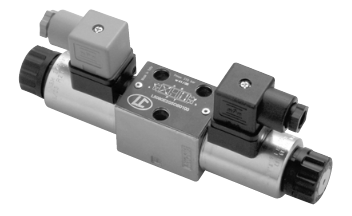
\includegraphics[width=0.6\textwidth]{../../figures/43-valve-real.png}\\
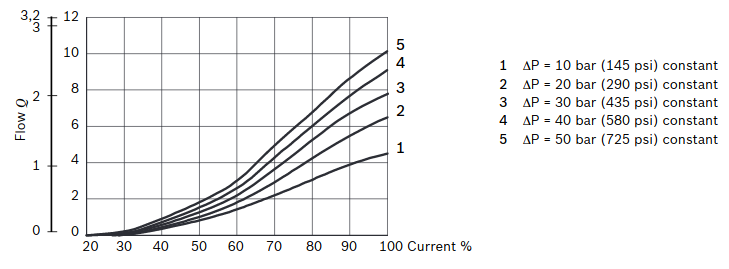
\includegraphics[width=0.99\textwidth]{../../figures/43-valve-current.png}\\
\end{center}
{\footnotesize Fuente: Bosch Rexroth}
\end{column}
\end{columns}
\end{frame}

\section{Block diagram}
\label{sec:org4bbe226}


\begin{frame}[label={sec:org95335cb}]{6. Diagrama de bloque - básico}
\begin{center}
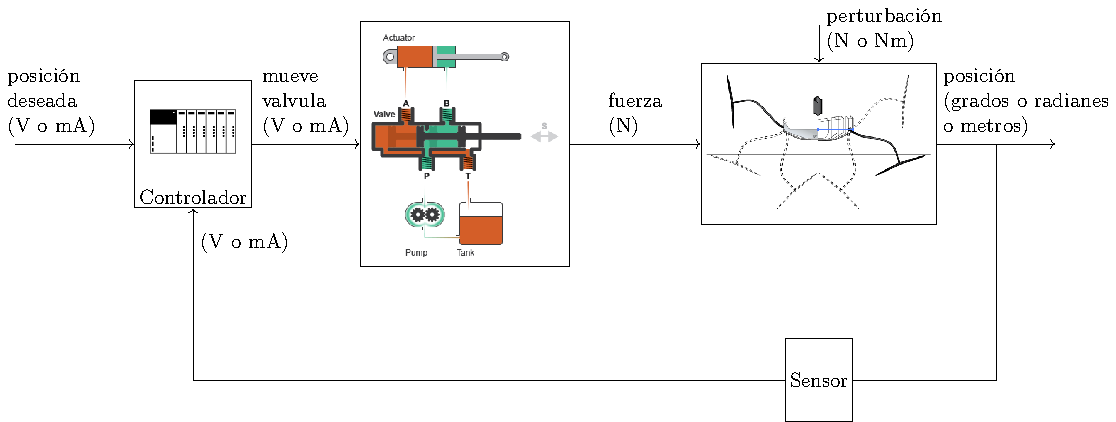
\includegraphics[width=1.0\textwidth]{../../figures/ac75-control-block-feedback-units}
\end{center}
\end{frame}


\begin{frame}[label={sec:orgbc7f7d6}]{\ldots{} y más elaborada}
\begin{center}
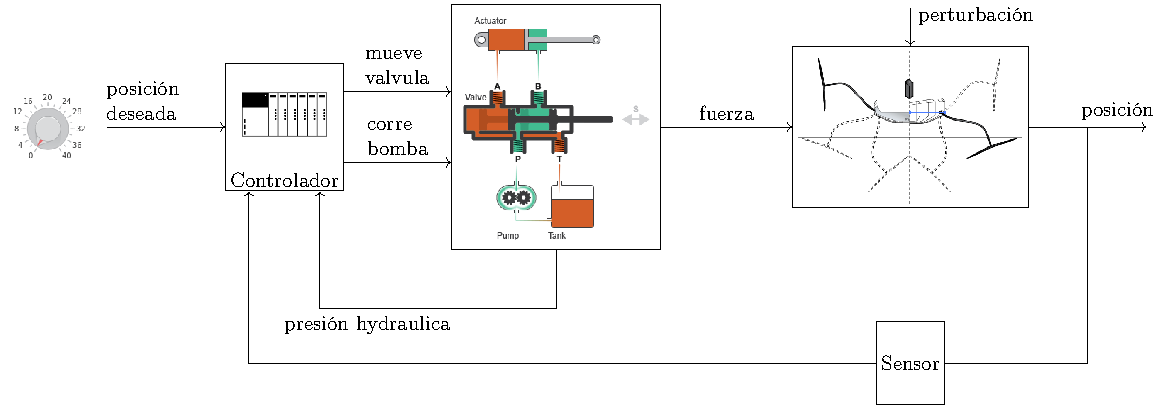
\includegraphics[width=.99\textwidth]{../../figures/ac75-control-block-details}
\end{center}
\end{frame}

\section{Control}
\label{sec:orgd23b6a0}

\begin{frame}[label={sec:org2101103}]{Sistema de control}
\begin{center}
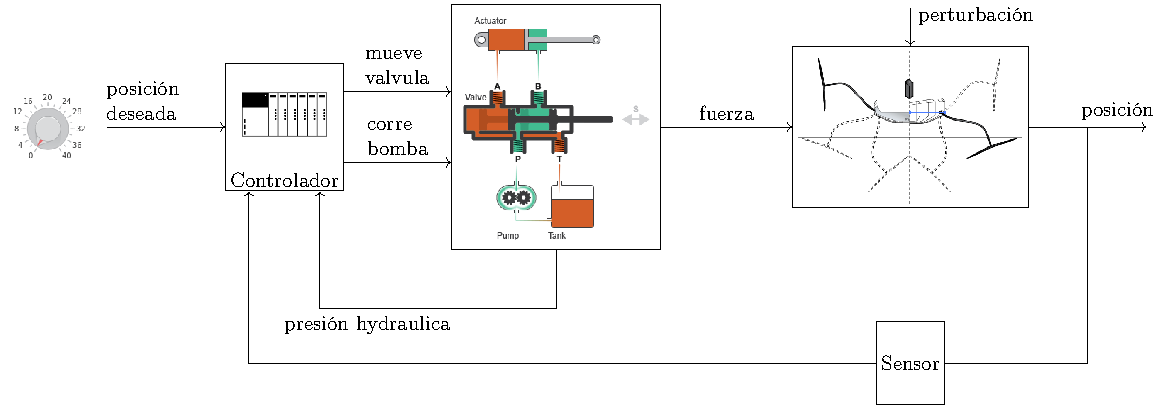
\includegraphics[width=.56\textwidth]{../../figures/ac75-control-block-details}
\end{center}

\begin{center}
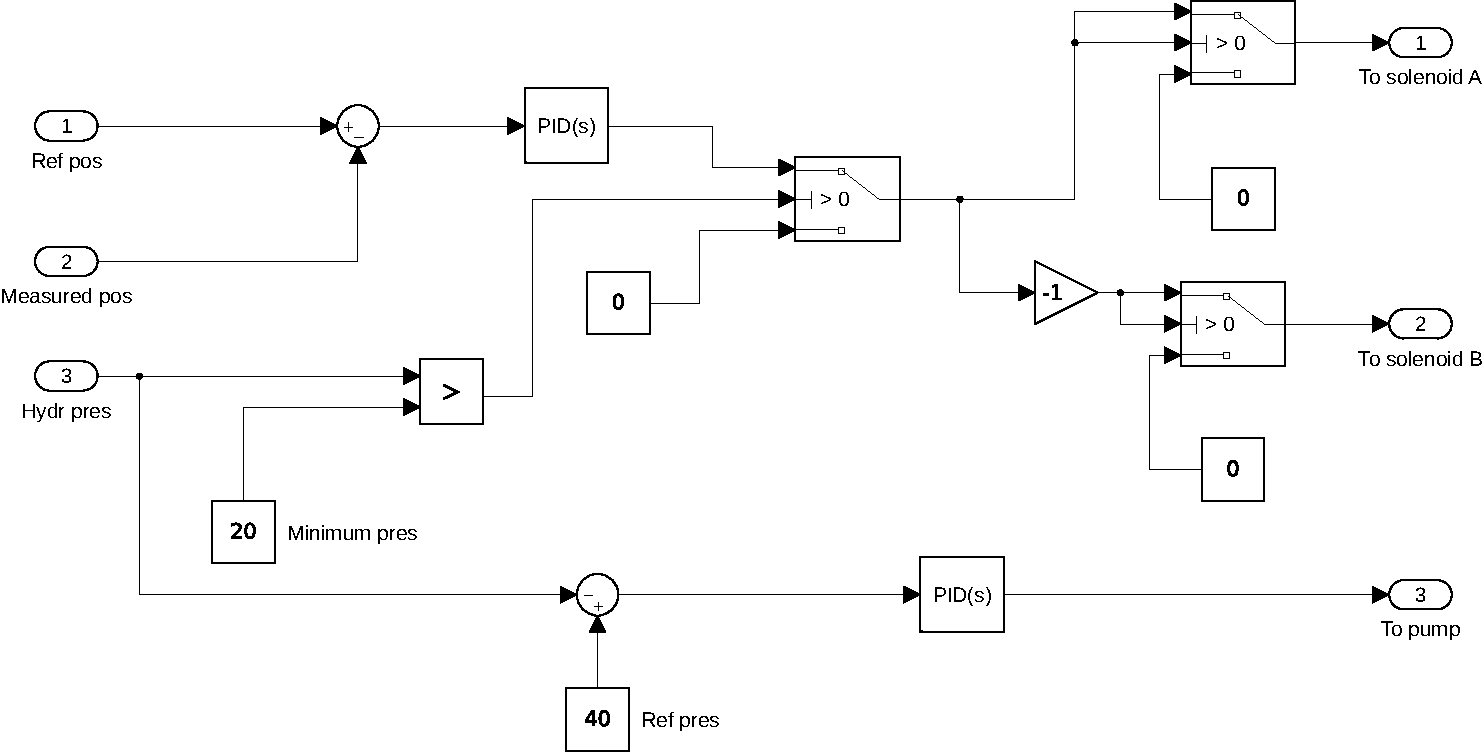
\includegraphics[width=.7\textwidth]{../../figures/ac75_control}
\end{center}
\end{frame}
\end{document}